Das LC-Display des Druckers erlaubt es, einige simple Einstellungen vor bzw. während des Druckens zu modifizieren, um eventuell Fehler zu beheben, den Drucker zu kalibrieren, etc. Da diese Einstellungen durchaus nützlich sein können, sollen hier die wichtigsten dar gestellt werden. \emph{(Notiz: Das eigentlische Starten/Stoppen eines Druckes wird über das OctoPrint Webinterface getan. Normalerweise ist die Verwendung des LC-Display nicht nötig.)}

\subsubsection{Aufbau des LCD-Menü:}
Das Menü des Druckers ist wie folgt aufgebaut:
\begin{itemize}[noitemsep]
	\item Prepare (Nur vor eines Druckvorganges)
	\begin{itemize}[noitemsep]
		\item Autostart (nur mit SD-Karte)
		\item Disable Steppers
		\item Auto-Home
		\item Preheat PLA
		\item Preheat ABS
		\item Cooldown
		\item Move axis
		\begin{itemize}
			\item Move 10mm 
			\item Move 1mm
			\item Move 0.1mm
		\end{itemize}
	\end{itemize}
	\item Tune (Nur während eines Druckvorganges)
	\begin{itemize}[noitemsep] 
		\item Speed
		\item Nozzle
		\item Bed
		\item Fan speed
		\item Flow
		\item Babystep X/Y/Z
		\item Change Filament
	\end{itemize}
	\item Control
	\begin{itemize}[noitemsep]
		\item Temperature
			\subitem Nozzle
			\subitem Bed
			\subitem Fan Speed
			\subitem \vdots
		\item \hspace{0.1pt} \vdots
	\end{itemize}
\end{itemize}
\emph{(Notiz: Einige Menüelemente wurden der Vereinfachung wegen nicht mit aufgelistet. Sie dienen rein der Feinsteuerung einiger Elemente des Druckers, und sollten nicht verändert werden!)}


Im Folgenden werden nun die wichtigsten Aktionen für die Interaktion mit dem Drucker aufgelistet, zusammen mit einigen Bildern der einzelnen Schritte.
\subsubsection{Änderung der Temperatur:}
Um die Temperatur des Druckers während des Druckvorganges zu ändern, können zwei Wege gewählt werden: Entweder die direkte Eingabe der neuen Werte in das Webinterface des Druckers, oder mithilfe des LC-Display. Zweiteres wird folgendermaßen erledigt:
\begin{enumerate}[noitemsep]
\item Auswählen des Menüpunktes "`Tune"' (während eines Druckes) oder "`Control"' (vor dem Druck)
\subitem Wurde "`Control"' ausgewählt muss nun "`Temperature"' gewählt werden.
\item Zur Änderung der Temperatur des Bettes nimmt man den Punkt "`Bed"', zur Änderung der Düsentemperatur den Punkt "`Nozzle"':\\
\begin{center}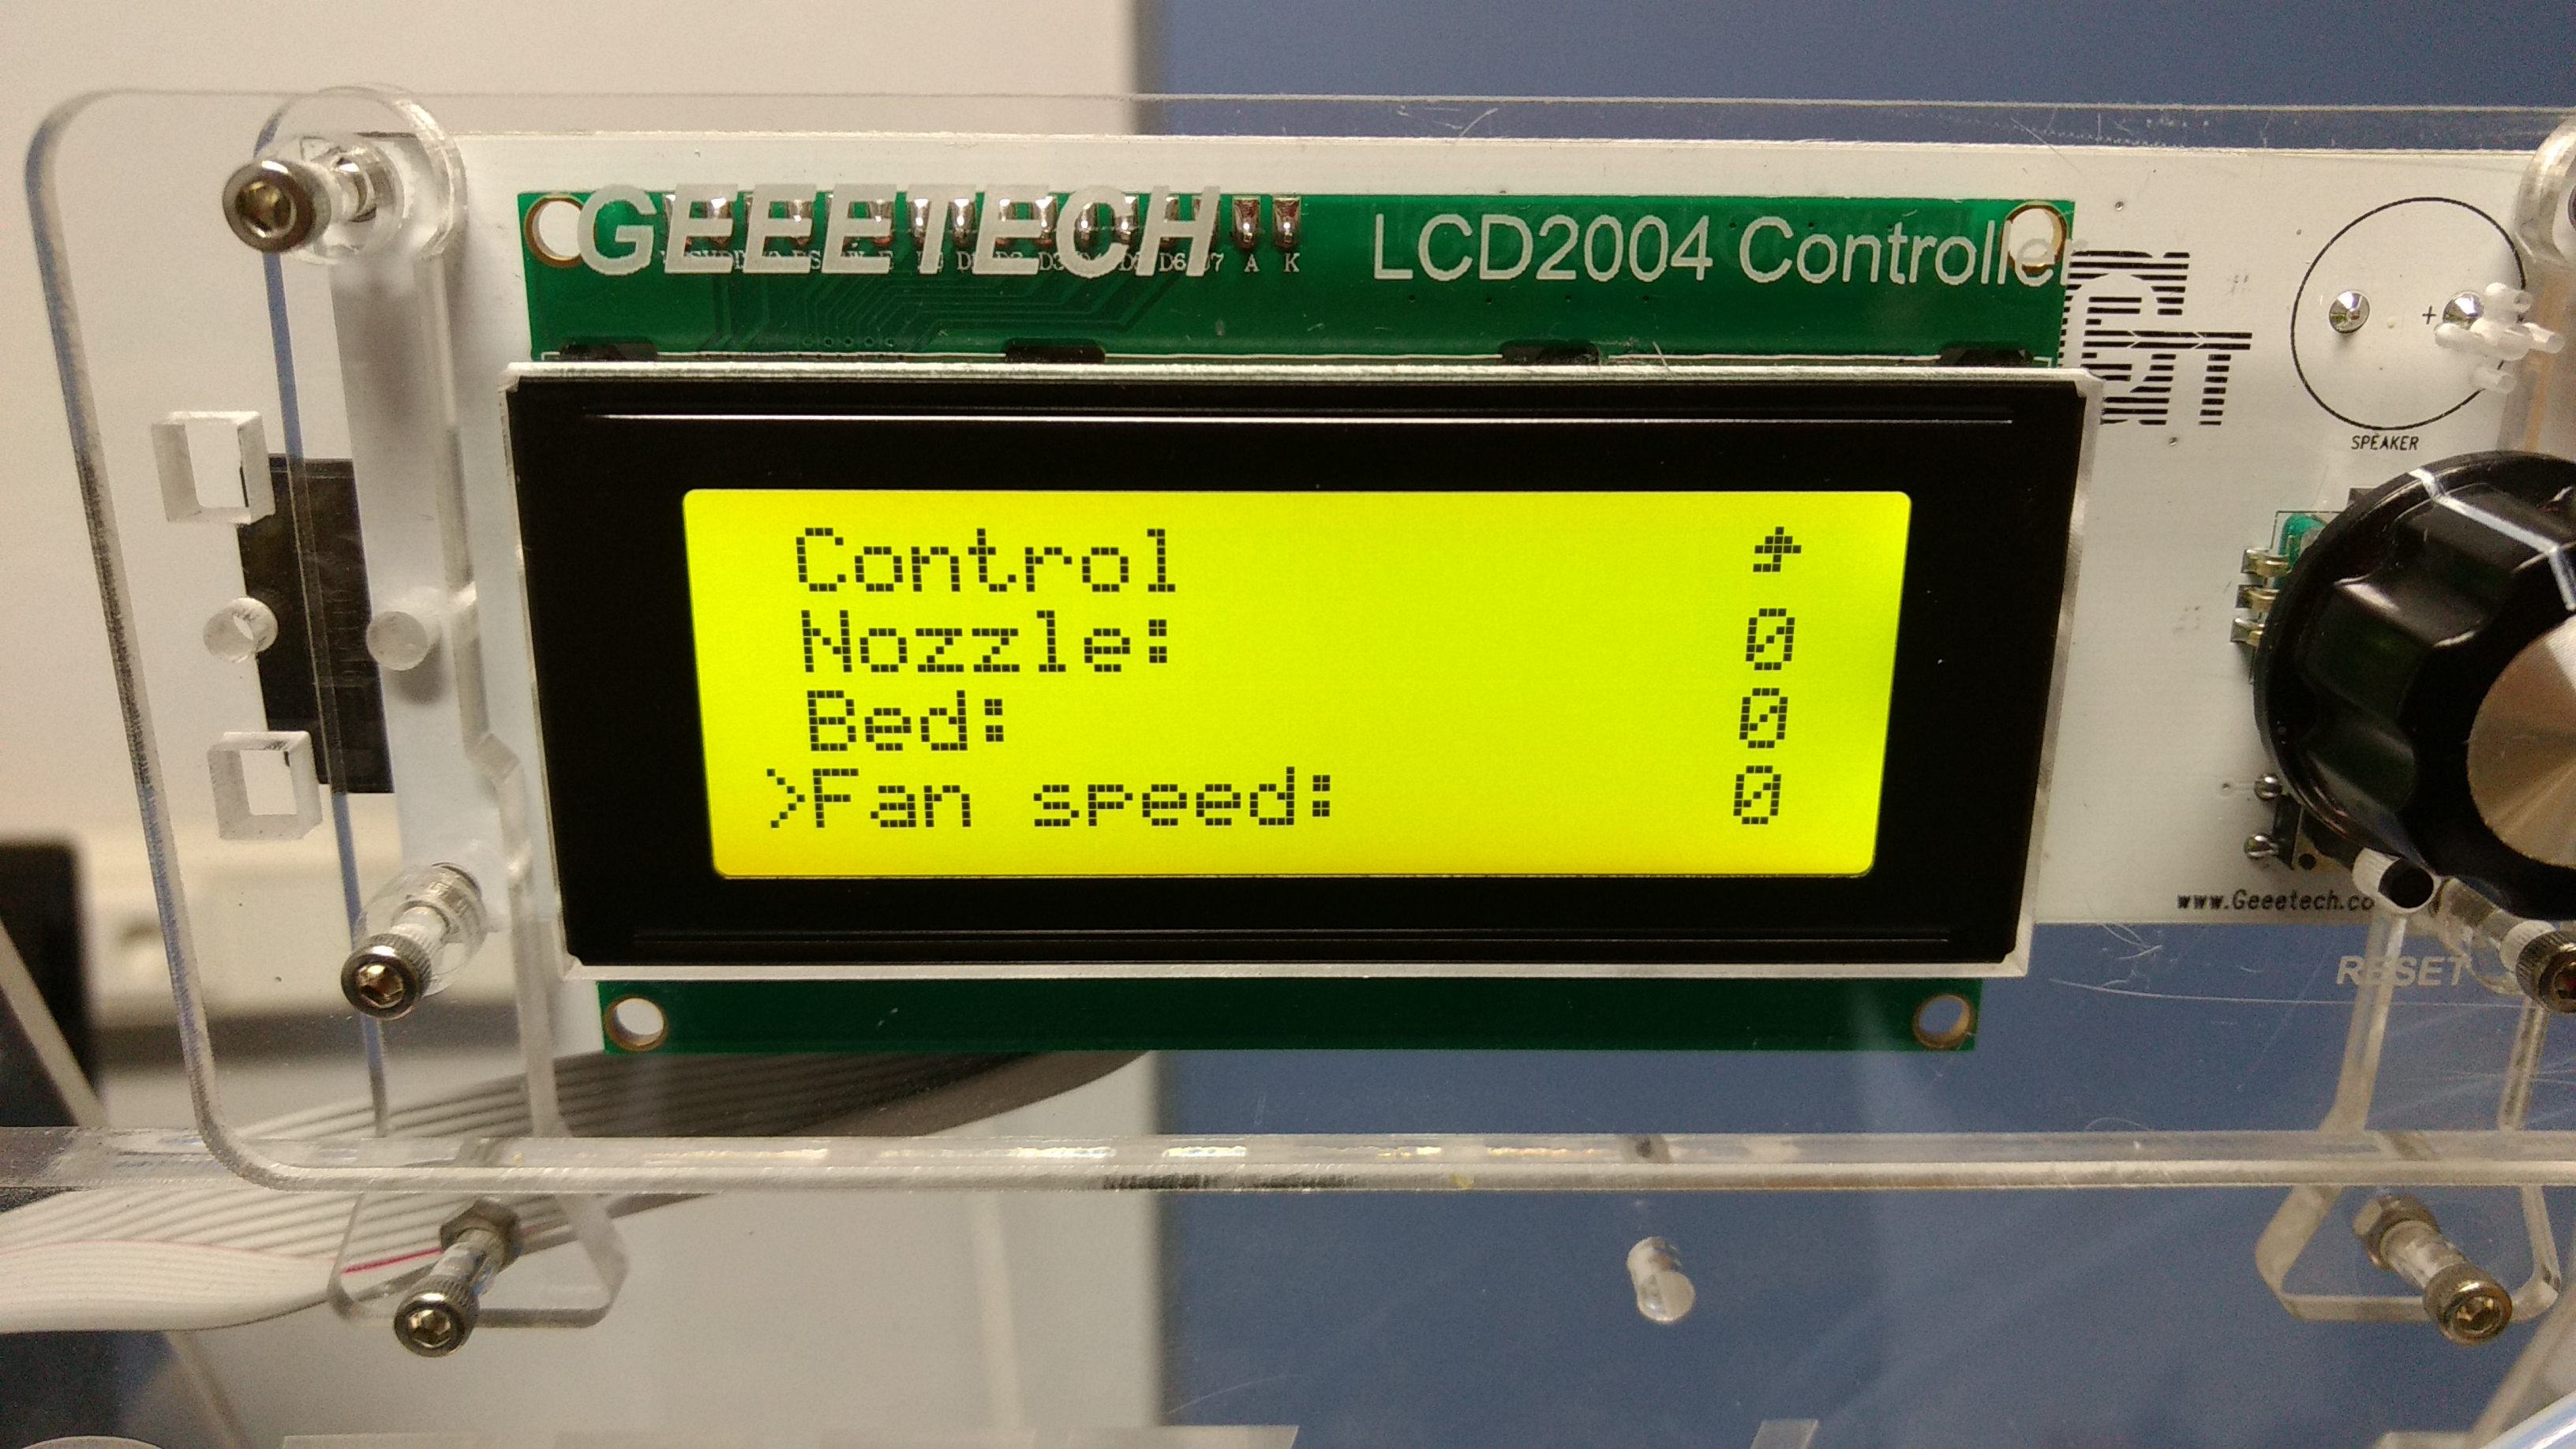
\includegraphics[width=0.5\textwidth]{Bilder/Tutorial/IMG_20161101_143633204.jpg}\end{center}
\item Nun stellt man die gewünschte neue Temperatur mithilfe des Drehknaufes ein, und bestätigt mit einem Druck auf den Knopf.
\end{enumerate}
Die neu eingestellte Temperatur wird nun ausgewählt, und von der Steuerelektronik eingeregelt, welches auf dem Info-Screen dar gestellt wird:\\
\begin{center}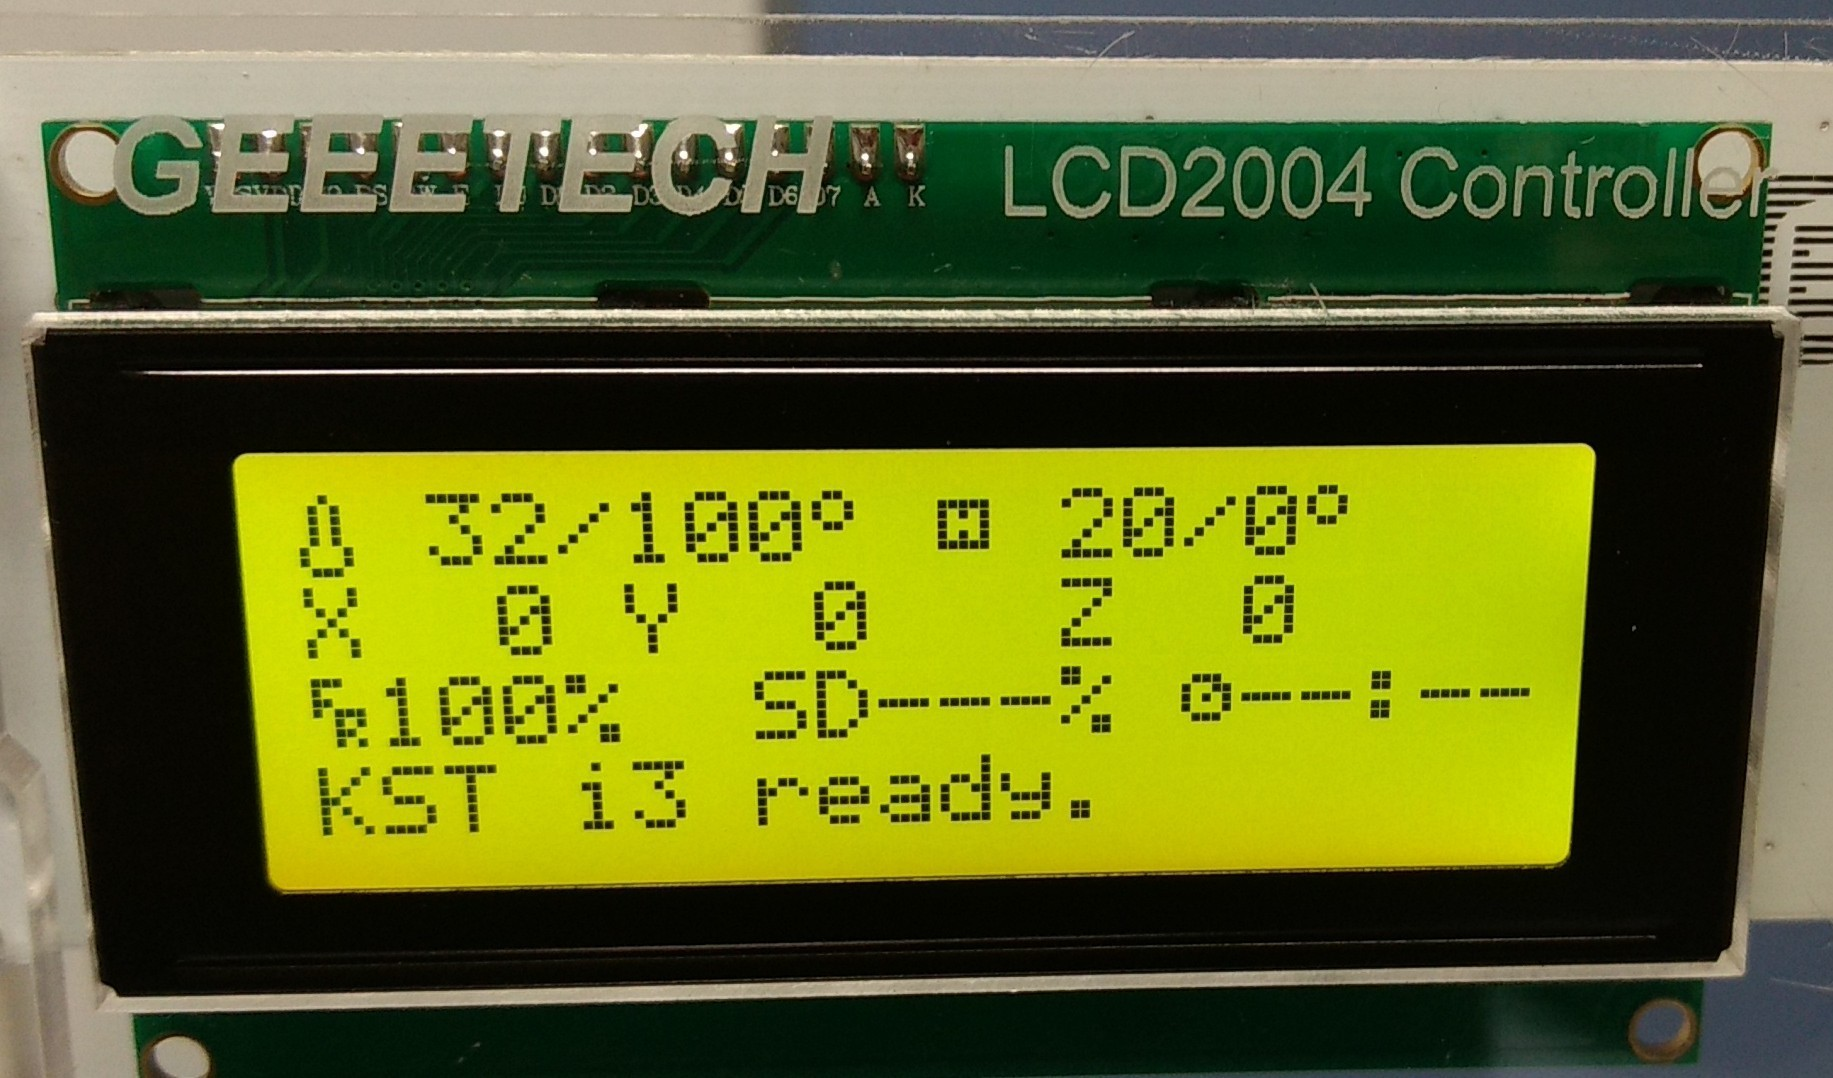
\includegraphics[width=0.5\textwidth]{Bilder/Tutorial/IMG_20161101_143426156.jpg}\end{center}